% 1977 年江苏苏州市初试卷第 6 题：MT 是 ⊙O 的切线，T 为切点，
% O、P、A、M 依次在同一直线上，TP⊥MO 交于 P（按源卷第 3 页布局）
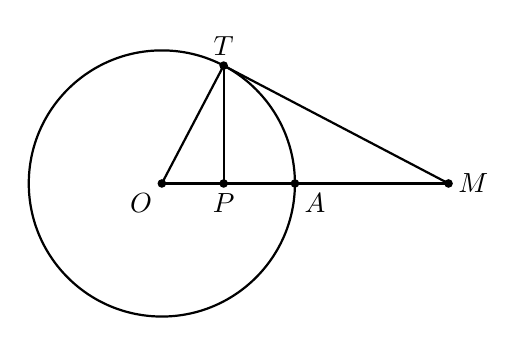
\begin{tikzpicture}[scale=1.3]
  \coordinate (O) at (0,0);
  \coordinate (M) at (2.8,0);
  \coordinate (A) at (1.3,0);
  \coordinate (P) at (0.6036,0);
  \coordinate (T) at (0.6036,1.1514);
  \draw[thick] (O) circle (1.3);
  \draw[thick] (O) -- (M);
  \draw[thick] (O) -- (T);
  \draw[thick] (T) -- (M);
  \draw[thick] (T) -- (P);
  \fill (O) circle (1.2pt) node[below left] {$O$};
  \fill (P) circle (1.2pt) node[below] {$P$};
  \fill (A) circle (1.2pt) node[below right] {$A$};
  \fill (M) circle (1.2pt) node[right] {$M$};
  \fill (T) circle (1.2pt) node[above] {$T$};
\end{tikzpicture}
